% Preamble
\documentclass[11pt]{article}

% Packages
\usepackage{amsmath}
\usepackage{amssymb}
\usepackage{tikz}
\usetikzlibrary{arrows,arrows.meta,positioning,calc,petri}
\usepackage{adjustbox}
\usepackage{enumitem}
\usepackage{listings}
\usepackage[ruled,vlined]{algorithm2e}
\SetKwRepeat{Do}{do}{until}%
\newtheorem{theorem}{Theorem}

% Document
\begin{document}

    \section*{Rule O: Inhibited transition}\label{sec:rule_o}
    We can find the lower bound of tokens at a place $p_0$.
    Any inhibitor arc from $p_0$ with a weight smaller than the lower bound
    always inhibits the given transition, which means that the transition can be removed.
    See Figure~\ref{fig:rule_o} for a formal description of Rule~O.

    \begin{figure}[h!]
        \centering
        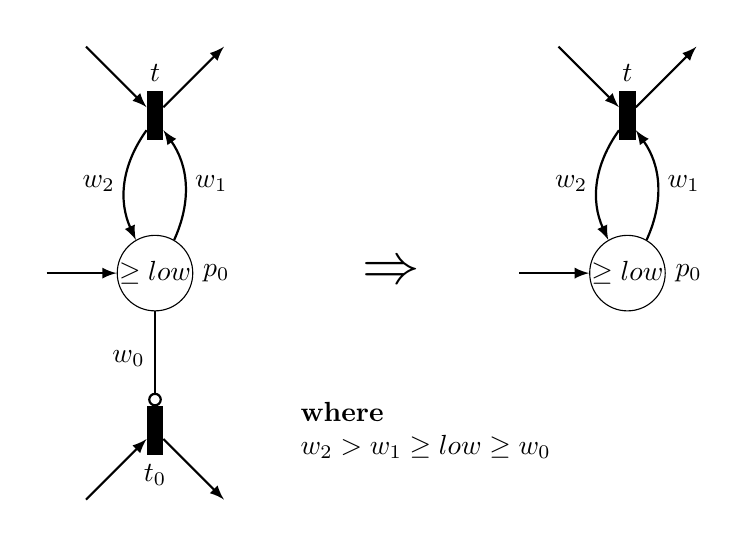
\begin{tikzpicture}
            % Left side places
            \node[place,label=right:$p_0$] (place1) at (0,0) {$\geq low$};

            % Left side transition
            \node[transition,minimum height=6mm,minimum width=2mm,fill=black,label=above:$t$] (negTrans1) at (0,2) {};
            \node[transition,minimum height=6mm,minimum width=2mm,fill=black,label=below:$t_0$] (remTrans1) at (0,-2) {};

            % Left side invisible nodes
            \node (negIn1) at (-1,3) {};
            \node (negOut1) at (1,3) {};
            \node (placeIn1) at (-1.5,0) {};
            \node (remIn1) at (-1,-3) {};
            \node (remOut1) at (1,-3) {};

            % Left side arcs between transitions and nodes
            \draw[-latex,thick] (negTrans1) edge[bend right] node[left] {$w_2$} (place1);
            \draw[-latex,thick] (place1) edge[bend right] node[right] {$w_1$} (negTrans1);
            \draw[-{Circle[open]},thick] (place1) -- node[left] {$w_0$} (remTrans1);

            % Left side arcs to/from invisible nodes
            \draw[-latex,thick] (negIn1) -- (negTrans1);
            \draw[-latex,thick] (negTrans1) -- (negOut1);
            \draw[-latex,thick] (placeIn1) -- (place1);
            \draw[-latex,thick] (remIn1) -- (remTrans1);
            \draw[-latex,thick] (remTrans1) -- (remOut1);

            % ================== Middle arrow ==================
            \node (arrow) at (3,0) {\huge$\Rightarrow$};
            \node[text width=3.5cm] at (3.6, -2) {\textbf{where}\\$w_2>w_1\geq low\geq w_0$};
            % ==================================================

            % Right side places
            \node[place,label=right:$p_0$] (place2) at (6,0) {$\geq low$};

            % Right side transitions
            \node[transition,minimum height=6mm,minimum width=2mm,fill=black,label=above:$t$] (negTrans2) at (6,2) {};

            % Right side invisible nodes
            \node (negIn2) at (5,3) {};
            \node (negOut2) at (7,3) {};
            \node (placeIn2) at (4.5,0) {};

            % Right side arcs between places and transition
            \draw[-latex,thick] (negTrans2) edge[bend right] node[left] {$w_2$} (place2);
            \draw[-latex,thick] (place2) edge[bend right] node[right] {$w_1$} (negTrans2);

            % Right side arcs to/from invisible nodes
            \draw[-latex,thick] (negIn2) -- (negTrans2);
            \draw[-latex,thick] (negTrans2) -- (negOut2);
            \draw[-latex,thick] (placeIn2) -- (place2);

        \end{tikzpicture}
        \vspace{1cm}

        \begin{adjustbox}{center}
            \begin{tabular}{|p{80mm}|p{45mm}|} \hline
            Precondition & Update \\ \hline
            Fix place $p_0$ and transition $t_0$ s.t.:
            \begin{itemize}[leftmargin=10mm]
                \item[O1)] $t_0\in p_0^\circ$
                \item[O2)] $I(p_0,t_0)\leq low$
            \end{itemize}
            where
            \[
                low=\min\{M_0(p_0)\}\cup\{\boxplus(p_0, t)\mid t\in p_0^\boxminus\}
            \]
            &
            \begin{itemize}[leftmargin=10mm]
                \item[UO1)] Remove $t_0$.
            \end{itemize} \\ \hline
            \end{tabular}
        \end{adjustbox}
        \caption{Rule O: Inhibited transition}
        \label{fig:rule_o}
    \end{figure}

    \begin{theorem}
        Rule~O in Figure~\ref{fig:rule_o} is correct for CTL*
    \end{theorem}

\end{document}
